\documentclass[10pt,letterpaper]{article}

\usepackage[margin=1in]{geometry}
\usepackage{iftex}
% mathptmx has no TU-encoded faces, so under XeTeX (Tectonic) earlier versions fell back
% to Latin Modern regular and lost every bold and italic. Use Termes there.
\ifPDFTeX\usepackage{mathptmx}\else\usepackage{fontspec}\setmainfont{texgyretermes}[Extension=.otf,UprightFont=*-regular,BoldFont=*-bold,ItalicFont=*-italic,BoldItalicFont=*-bolditalic]\fi
\usepackage{amsmath}
\usepackage{amssymb}
\usepackage{graphicx}
\usepackage{booktabs}
\usepackage{listings}
\usepackage{xcolor}
\usepackage{tikz}
\usetikzlibrary{positioning,arrows.meta,fit,backgrounds,calc}
\usepackage{natbib}
\usepackage[colorlinks=true,linkcolor=blue,citecolor=blue,urlcolor=blue]{hyperref}
\usepackage{microtype}
\usepackage{parskip}
\usepackage{titlesec}
\usepackage{enumitem}
\usepackage{caption}

\setlength{\parskip}{6pt}
\setlength{\parindent}{0pt}
\setlength{\emergencystretch}{3em}

\lstset{
  basicstyle=\small\ttfamily,
  breaklines=true,
  frame=single,
  numbers=left,
  numberstyle=\tiny,
  xleftmargin=2em,
  framexleftmargin=1.5em,
  backgroundcolor=\color{gray!8},
}

\title{\textbf{TRACE: Trust, Runtime Attestation, and Compliance Evidence}\\
  \large A Portable Attestation Format for AI Agent Runtime Governance}

\author{
  Rishabh Poddar \quad Aaron Fulkerson \quad Imran Siddique \\
  OPAQUE Systems \\[4pt]
  \normalsize \url{https://github.com/agentrust-io/trace-spec}
}

\date{October 1, 2026 \\ \small Technical report, version 3}

\begin{document}

\maketitle

\begin{abstract}
TRACE (Trust, Runtime Attestation, and Compliance Evidence) proposes a
portable record for claims about AI agent runtimes: workload identity, model,
policy, data class, tool transcript, build provenance, and appraisal. It composes
RATS/EAT, signatures, and transparency evidence into a format that a relying party
can evaluate against its own trust policy. A valid signature establishes integrity
and possession of the signing key; hardware origin additionally requires verified
attestation and a binding from that evidence to the key. This technical report
describes the original design and preserves the recorded software evaluation of
agentrust-trace (trace-spec revision 523f8cc, whose signing code is release
0.3.0) and trace-tests 0.2.0. The evaluation measures
canonicalization, Ed25519 signing and verification, record size, and fixture
outcomes. It does not measure silicon certificate-chain appraisal or establish
that the recorded runtime claims are true. The current normative specification
and its implementation limits are maintained separately.
\end{abstract}

\paragraph{Scope of this edition.}
This is an author-prepared technical report, not peer reviewed and not a
normative specification. It revises a manuscript originally dated June 23, 2026;
the recorded experiments include later runs and have not been rerun for this
edition. Architectural requirements describe intended checks, not proof that
the historical SDK implements every check. Consult the linked project
specification and limitations before implementing the design.
Version 3 (October 1, 2026) corrects the identification of the evaluated SDK, states that the
evaluated vectors and checker use the v0.1 profile URI, narrows the
conformance-module descriptions to what the evaluated checks do, fixes the
install command, corrects five bibliography entries, replaces a vendor
model name in the worked example, and restores bold and italic type that the
Tectonic build had dropped; the recorded numbers are unchanged. Version
2 corrected one sentence in the related-work discussion
of transparency logs, which implied that log registration makes omitted events
detectable.

\tableofcontents
\newpage

\section{Introduction}
\label{sec:intro}

AI agents now invoke tools, call external services, and exchange data across
organizational boundaries. When a relying party (a downstream service, an auditor,
or a partner organization) consumes the result of an agent workflow, it has
no portable, vendor-neutral way to answer basic governance questions: which policy
governed the agent, which identity was authenticated, what hardware enforced the
policy, and whether the recorded evidence has been altered. Ad hoc logs are
operator-controlled and therefore not trustworthy across a trust boundary.

TRACE (Trust, Runtime Attestation, and Compliance Evidence) is a signed, hardware-
attestable evidence record for AI agent runtimes. It instantiates the RATS
roles~\citep{rats2021} (Attester, Verifier, Relying Party) and profiles the
Entity Attestation Token~\citep{eat2023} with the fields an agent runtime needs:
the model and runtime measurements, the policy and data class in effect, the
invoked-tool transcript, the authenticated agent identity, a confirmation key
rooted in the TEE attestation, and an inclusion proof on an append-only
transparency log. The result, a \emph{Trust Record}, is appraisable offline,
without trusting the operator that produced it.

\subsection*{Contributions}

\begin{itemize}[leftmargin=1.5em]
  \item \textbf{A portable evidence record.} The Trust Record: an EAT profile that
    binds model, runtime, policy, data class, tool transcript, identity, a
    confirmation key, and a transparency receipt into one signed artifact
    (Section~\ref{sec:model}).
  \item \textbf{A role and protocol model.} How Attester, Verifier, and Relying
    Party interact in the RATS passport model, for single- and cross-organizational
    deployments (Section~\ref{sec:protocol}).
  \item \textbf{An offline verification procedure.} Signature binding, freshness,
    silicon-root chaining, reference-value matching, policy, transparency, and
    provenance, with no callback to the issuer (Section~\ref{sec:verification}).
  \item \textbf{A reference profile and conformance suite.} cMCP~\citep{cmcp2026}
    produces Trust Records at the MCP boundary (Section~\ref{sec:profiles}), and a
    conformance suite checks records against the normative requirements
    (Section~\ref{sec:conformance}).
\end{itemize}

\subsection*{Paper structure}

Section~\ref{sec:background} reviews RATS, EAT, TEE attestation, and agent identity.
Section~\ref{sec:model} defines the Trust Record. Section~\ref{sec:protocol} gives
the role model and protocol. Section~\ref{sec:verification} specifies verification.
Section~\ref{sec:profiles} describes profiles, with cMCP as the reference instance.
Section~\ref{sec:conformance} describes the conformance suite,
Section~\ref{sec:related} surveys related work, and Section~\ref{sec:conclusion}
concludes.

\section{Background}
\label{sec:background}

\subsection{Remote Attestation (RATS)}

The RATS architecture~\citep{rats2021} separates three roles: the \emph{Attester}
produces evidence about a target environment; the \emph{Verifier} appraises that
evidence against policy and reference values to produce an attestation result; and
the \emph{Relying Party} consumes the result to make a trust decision. TRACE maps
the agent runtime to the Attester; the Trust Record carries both the runtime's
Evidence and the Verifier's appraisal (the \texttt{appraisal} claim, in the EAR
format) so a Relying Party can act on it offline. RATS describes two topologies: the
\emph{background-check} model, in which the Relying Party forwards Evidence to a
Verifier at decision time, and the \emph{passport} model, in which the Attester
obtains an appraised result up front and presents it directly. TRACE uses the
passport model: the Trust Record is self-contained and verifiable offline, so no
party need call back to the issuer.

\subsection{Entity Attestation Tokens (EAT)}

EAT~\citep{eat2023} standardizes a token carrying claims about an entity, including
measurements, a nonce, and a confirmation (\texttt{cnf}) key, in a JWT or CBOR-COSE
envelope. TRACE is an EAT profile under the URI
\texttt{tag:agentrust-io.com,2026:trace-v0.2}. It reuses the standard EAT claims
(\texttt{iat}, \texttt{nonce}, \texttt{cnf}, the profile claim) and adds the
agent-governance claims an agent runtime needs (\texttt{model}, \texttt{policy},
\texttt{data\_class}, \texttt{tool\_transcript}, \texttt{build\_provenance},
\texttt{appraisal}, \texttt{transparency}); these are enumerated in
Section~\ref{sec:model}.

\subsection{TEE Attestation}

Confidential-computing platforms (AMD SEV-SNP~\citep{amdsevsnp2023} and Intel
TDX~\citep{inteltdx2023}) produce hardware-signed reports binding a launch
measurement and a caller-supplied \texttt{report\_data} field. TRACE records the
measurement in \texttt{runtime} and binds the record's signing key through the
\texttt{cnf} claim; a profile additionally commits the key into \texttt{report\_data}
so the hardware report and the signing key are cryptographically linked (the cMCP
profile does this with an RFC~7638 JWK thumbprint, Section~\ref{sec:profiles}). The
\texttt{runtime.measurement} is the platform's launch measurement (for SEV-SNP
the 48-byte report measurement, for TDX the MRTD and runtime measurement registers),
which a verifier checks against vendor-published Reference Integrity Manifests
(RIMs) named by \texttt{runtime.rim\_uri}.

\subsection{Agent Identity}

SPIFFE/SVID~\citep{spiffe2018} provides workload identity that TRACE carries in the
\texttt{subject} claim (a SPIFFE ID or DID URI), so a record names \emph{which}
agent acted, not only \emph{which} enclave ran. The SVID is bound to the TEE
measurement, rooting identity in hardware; the companion Agent Manifest
specification~\citep{manifest2026} supplies the issuer keys and the
manifest-to-session binding behind that identity.

\subsection{The gap}

Each layer above exists, but none, alone, lets a relying party verify agent runtime
governance across a trust boundary. Static documentation (model cards, AIBOMs)
diverges from deployed reality; operational logs are self-reported and mutable;
hardware attestation proves the environment is genuine but says nothing about policy,
data class, or tools; content provenance is silent on execution. No open, portable,
vendor-neutral artifact binds \emph{what ran}, \emph{under what policy}, \emph{on
what data}, \emph{invoking which tools} into one record a third party can appraise
offline. TRACE closes that gap.

\section{The Trust Record}
\label{sec:model}

The unit of evidence in TRACE is the \emph{Trust Record}: a single signed artifact
that binds \emph{what executed} (model, code, runtime), \emph{under what policy},
\emph{on what data class}, \emph{invoking which tools}, optionally accompanied by attestation evidence. A record travels with the workload
across hosts, clouds, and providers. Offline checks require the relevant trusted
keys and evidence; a signature alone does not establish silicon provenance.

\subsection{Logical schema}

A Trust Record is an EAT~\citep{eat2023} carrying the claims in
Table~\ref{tab:fields}. All fields are required unless marked optional. The presence of a field does not verify its contents; appraisal requires
independent evidence and trust policy. Sub-records (for example per-tool-call transcripts)
compose under one root envelope.

\begin{table}[h]
\centering
\small
\caption{Trust Record claims (TRACE v0.2). ``Source primitive'' names the existing
standard each claim is drawn from; TRACE adds the binding into a hardware-attested
envelope rather than redefining the primitive.}
\label{tab:fields}
\begin{tabular}{p{2.9cm}p{6.2cm}p{3.4cm}}
\toprule
Field & Description & Source primitive \\
\midrule
\texttt{eat\_profile} & Profile URI identifying a TRACE v0.2 record:
  \texttt{tag:agentrust-io.com,2026:trace-v0.2} & EAT profile claim \\
\texttt{iat} & Issued-at timestamp (Unix epoch) & EAT standard claim \\
\texttt{subject} & Workload identity (agent, tool, or model invocation) &
  SPIFFE SVID or DID URI \\
\texttt{model} & Model identity, weights digest, version & EAT claim + AIBOM ref \\
\texttt{runtime} & TEE measurement chain (firmware $\rightarrow$ kernel
  $\rightarrow$ image $\rightarrow$ workload) & RATS Evidence + vendor RIM \\
\texttt{policy} & Bound policy-set hash and enforcement mode &
  Policy hash sealed to TEE measurement \\
\texttt{data\_class} & Classification of inputs and outputs &
  Per-call classification label \\
\texttt{tool\_transcript} & \emph{(optional)} Tool calls invoked, parameters
  classified, responses filtered & MCP / A2A transcript, bound by hash \\
\texttt{build\_provenance} & How the running code and model were built &
  SLSA Provenance v1.0 \\
\texttt{appraisal} & Verifier's appraisal of the evidence & EAR (AR4SI) \\
\texttt{transparency} & Inclusion proof on an append-only log & SCITT receipt URI \\
\texttt{cnf} & Confirmation key binding the record to a TEE-held signing key &
  EAT \texttt{cnf} claim (RFC 7800) \\
\texttt{signature} & \emph{(optional field)} Embedded signature; see
  Section~\ref{sec:model:sig} & JWS / COSE over canonical JSON \\
\bottomrule
\end{tabular}
\end{table}

\subsection{Claim structure}

The composite claims carry the following members (optional members italicized):

\begin{itemize}[leftmargin=1.5em]
  \item \textbf{\texttt{model}}: \texttt{provider}, \texttt{model\_id},
    \emph{\texttt{version}}, \emph{\texttt{weights\_digest}},
    \emph{\texttt{aibom\_uri}}.
  \item \textbf{\texttt{runtime}}: \texttt{platform} (one of \texttt{intel-tdx},
    \texttt{amd-sev-snp}, \texttt{nvidia-h100}, \texttt{nvidia-blackwell},
    \texttt{aws-nitro}, \texttt{arm-cca}, \texttt{google-confidential-space},
    \texttt{tpm2}, \texttt{software-only}), \texttt{measurement} (a
    \texttt{sha256:}/\texttt{sha384:} digest), \emph{\texttt{rim\_uri}},
    \emph{\texttt{nonce}}, \emph{\texttt{firmware\_version}}.
  \item \textbf{\texttt{policy}}: \texttt{bundle\_hash},
    \texttt{enforcement\_mode} (\texttt{enforce} $|$ \texttt{advisory} $|$
    \texttt{silent}), \emph{\texttt{version}}, \emph{\texttt{policy\_uri}}.
    \texttt{enforcement\_mode} MUST default to \texttt{enforce}; \texttt{silent}
    MUST be configured explicitly.
  \item \textbf{\texttt{tool\_transcript}}: \texttt{hash} (binds the full
    transcript), \emph{\texttt{call\_count}}, \emph{\texttt{transcript\_uri}}.
  \item \textbf{\texttt{build\_provenance}}: \texttt{slsa\_level} (0 to 3),
    \emph{\texttt{builder}}, \texttt{digest}, \emph{\texttt{provenance\_uri}}.
  \item \textbf{\texttt{appraisal}}: \texttt{status} (\texttt{affirming} $|$
    \texttt{warning} $|$ \texttt{contraindicated} $|$ \texttt{none}),
    \texttt{verifier}, \emph{\texttt{policy\_ref}}, \emph{\texttt{timestamp}}.
  \item \textbf{\texttt{cnf}}: a single \texttt{jwk} (\texttt{kty}, and the key
    material required by the key type, e.g. \texttt{crv}/\texttt{x} for OKP,
    \texttt{crv}/\texttt{x}/\texttt{y} for EC).
\end{itemize}

The three questions a deployer must answer map onto these claims:
\texttt{runtime}$+$\texttt{model}$+$\texttt{build\_provenance} answer \emph{what
ran}; \texttt{tool\_transcript} answers \emph{what it did}; \texttt{policy}$+$
\texttt{data\_class} answer \emph{what rules were in force}.

\subsection{Wire format}

The envelope is an EAT~\citep{eat2023}: a JWT in JSON-friendly contexts, or a
CWT/CBOR-COSE in constrained or high-throughput contexts. The profile URI is
\texttt{tag:agentrust-io.com,2026:trace-v0.2}.

\subsection{Signature binding}
\label{sec:model:sig}

Every Trust Record MUST be cryptographically bound by a signature over its canonical
form, made by the key in \texttt{cnf}. Canonicalization is RFC~8785 (JCS):
ad-hoc sorting such as \texttt{json.dumps(sort\_keys=True)} is insufficient because
it diverges from JCS on non-ASCII strings and IEEE~754 number serialization. The
binding may be \emph{embedded} (the top-level \texttt{signature} field, base64url, over
the record with \texttt{signature} absent) or \emph{enveloping} (a JWS, a
\texttt{COSE\_Sign1}, or cMCP's RuntimeClaim). Each profile declares which it uses.
A record with no verifiable binding is not a Trust Record; verifiers MUST reject it,
and schema validity alone confers no trust. JWT contexts use \texttt{ES256},
\texttt{ES384}, or \texttt{EdDSA}; COSE contexts use \texttt{COSE\_Sign1} or
\texttt{COSE\_Sign}.

\subsection{Freshness}

Records MUST carry \texttt{iat}, and verifiers MUST enforce a maximum age (default
24~hours; a profile MAY override). For online verification, a verifier MAY supply a
challenge nonce that the issuer echoes in \texttt{runtime.nonce}; when a challenge
was issued, a record that omits or mismatches it MUST be rejected.

\subsection{Worked example}

A Trust Record in the readable (JWT) form, abbreviated:

\begin{lstlisting}
{
  "eat_profile": "tag:agentrust-io.com,2026:trace-v0.2",
  "iat": 1750676142,
  "subject": "spiffe://trust.example.org/agent/payments-processor/prod",
  "model":   { "provider": "example-provider", "model_id": "example-model",
               "version": "20251001", "weights_digest": "sha256:a3f8d2c1..." },
  "runtime": { "platform": "amd-sev-snp", "measurement": "sha384:c9e4b1d2...",
               "rim_uri": "https://kdsintf.amd.com/vcek/v1/Milan/..." },
  "policy":  { "bundle_hash": "sha256:b2c3d4e5...", "enforcement_mode": "enforce",
               "version": "1.2.0" },
  "data_class": "confidential",
  "tool_transcript": { "hash": "sha256:d4e5f6a7...", "call_count": 3 },
  "build_provenance": { "slsa_level": 2,
               "builder": "https://github.com/slsa-framework/slsa-github-generator",
               "digest": "sha256:e5f6a7b8..." },
  "appraisal": { "status": "affirming", "verifier": "https://trust-authority.example.org" },
  "transparency": "https://registry.agentrust-io.com/claim/trace-2026-06-23T09:15:42Z-f2a8d1",
  "cnf": { "jwk": { "kty": "EC", "crv": "P-256", "x": "MEkwEw...", "y": "GHkVPy..." } }
}
\end{lstlisting}

The signature is carried per the binding the profile declares
(Section~\ref{sec:model:sig}); the cMCP profile wraps this record in a signed
RuntimeClaim (Section~\ref{sec:profiles}).

\subsection{External execution evidence}

A deployment may attach independent, out-of-band receipts to individual
audit-chain entries (for example, a signed assertion from a safety controller
confirming or rejecting an actuation). The Trust Record commits the audit chain by
hash; the receipts live inside that chain, not in the record. A receipt carries an
issuer identity (\texttt{issuer}), a key reference (\texttt{issuer\_key\_id}), a
signature over its canonical fields (\texttt{signature}), a content digest
(\texttt{evidence\_hash}), a type tag (\texttt{evidence\_type}), and a binding to the
tool call (\texttt{linked\_call\_id}). A verifier holding the issuer's key verifies
the signature over the canonical (JCS) receipt fields and asserts that
\texttt{linked\_call\_id} matches the enclosing entry; a failure invalidates the
record. A receipt whose issuer key is unknown is \emph{unverified, not invalid}: the
gateway-produced evidence stands, and the verifier surfaces an advisory status. TRACE
binds the receipt into the audit chain; it does not certify that the physical action
occurred or met any functional-safety standard: that claim belongs to the issuer.

\section{Roles and Protocol}
\label{sec:protocol}

\subsection{Roles}

TRACE instantiates the three RATS roles~\citep{rats2021}. The \emph{Attester} is the
agent runtime: it holds the TEE-bound signing key, gathers Evidence (the platform
measurement chain), and issues a Trust Record. The \emph{Verifier} appraises that
Evidence against reference values and policy and emits an appraisal (the record's
\texttt{appraisal} claim, in the EAR format). The \emph{Relying Party} (a
downstream service, an auditor, or a partner) consumes the record and the
appraisal to make a trust decision.

TRACE follows the RATS \emph{passport} model: the Attester obtains its evidence and
ships a self-contained Trust Record that travels with the workload. Any party
verifies it offline, with no callback to the issuer and no vendor in the trust path
beyond the silicon root and the transparency-log operator
(Section~\ref{sec:verification}).

\begin{figure}[h]
\centering
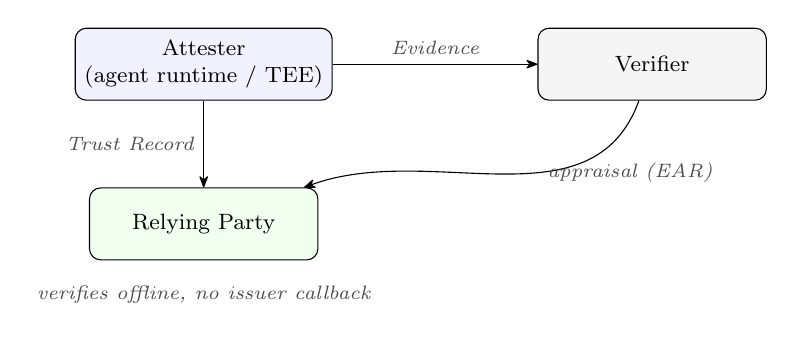
\begin{tikzpicture}[
  font=\footnotesize,
  >={Stealth[round]},
  role/.style={draw, rounded corners, align=center, minimum width=2.9cm, minimum height=2.6em},
  note/.style={font=\scriptsize\itshape, text=black!70},
]
\node[role, fill=blue!5] (att) {Attester\\(agent runtime / TEE)};
\node[role, fill=gray!8, right=2.6cm of att] (ver) {Verifier};
\node[role, fill=green!6, below=1.1cm of att] (rp) {Relying Party};

\draw[->] (att) -- node[note, above]{Evidence} (ver);
\draw[->] (ver) to[out=250,in=20] node[note, right, pos=0.4]{appraisal (EAR)} (rp);
\draw[->] (att) -- node[note, left]{Trust Record} (rp);
\node[note, below=0.2cm of rp] {verifies offline, no issuer callback};
\end{tikzpicture}
\caption{TRACE in the RATS passport model. The Attester ships a self-contained
Trust Record; the Verifier's appraisal travels in the record so the Relying Party
appraises it without contacting the issuer.}
\label{fig:roles}
\end{figure}

\subsection{Key hierarchy}

Signing keys form a chain rooted in silicon:
silicon root key (vendor-managed, hardware-bound) $\rightarrow$ platform attestation
key (Intel TDX Quote-signing key, AMD VCEK/VLEK, NVIDIA NRAS) $\rightarrow$ workload
attestation key (TEE-bound, ephemeral) $\rightarrow$ record-signing key (per
workload, optionally per session). The record-signing key is the one named in
\texttt{cnf}; workload-level keys SHOULD rotate at TEE-image boundaries, and
verifiers MUST consult current revocation status at verification time.

\subsection{Single-organization flow (Phase 1)}

\begin{enumerate}[leftmargin=1.5em]
  \item \textbf{Startup attestation.} The runtime launches inside a TEE, derives its
    record-signing key, and obtains a platform attestation report binding that key.
  \item \textbf{Issuance.} For each governed execution (an invocation, or a session),
    the runtime assembles a Trust Record (\texttt{model}, \texttt{runtime},
    \texttt{policy}, \texttt{data\_class}, \texttt{tool\_transcript},
    \texttt{build\_provenance}), signs it (Section~\ref{sec:model:sig}), and
    optionally registers it on the transparency log, filling \texttt{transparency}.
  \item \textbf{Appraisal and consumption.} A Verifier appraises the record and a
    Relying Party acts on it, both offline.
\end{enumerate}

Issuance granularity is profile-defined: the cMCP profile issues one record per
session, at session close, binding that session's audit chain; a profile that needs
finer evidence may issue per invocation. In all cases the \texttt{subject} is the
workload's SPIFFE identity~\citep{spiffe2018}, bound to the TEE measurement so the
record names which agent acted.

\subsection{Cross-organization flow (Phase 2)}

When two runtimes in different trust domains participate (for example a gateway
and an upstream server, each in its own TEE), each is an independent Attester. Each
produces its own Trust Record, signed by its own \texttt{cnf} key and bound to its
own platform attestation, and both carry the \emph{same} \texttt{subject}/session
identifier. The shared identifier links the two records without sharing private key
material; a Verifier confirms the linkage and appraises each record independently, so
tampering with one does not affect the other. cMCP~\citep{cmcp2026} demonstrates this
as a dual-TEE protocol at the MCP boundary.

\begin{figure}[h]
\centering
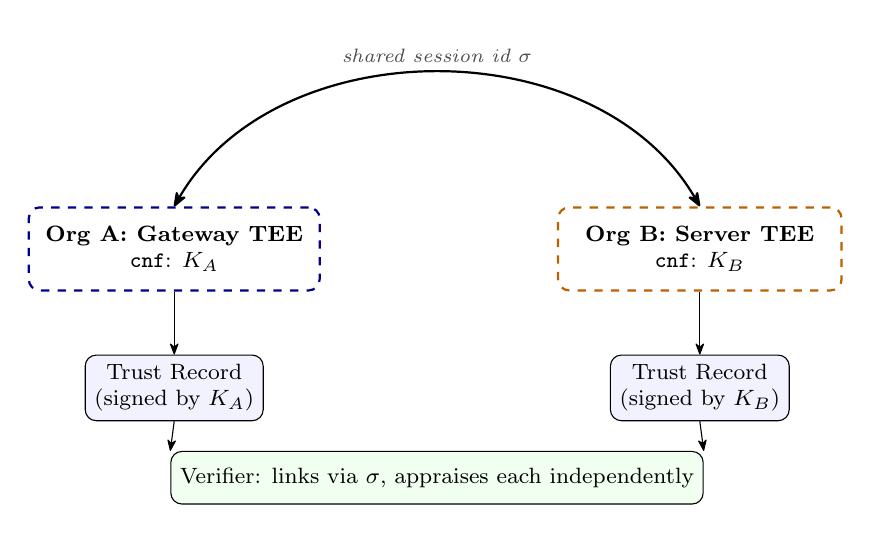
\begin{tikzpicture}[
  font=\footnotesize,
  >={Stealth[round]},
  tee/.style={draw, dashed, thick, rounded corners, align=center, minimum width=3.6cm, minimum height=3.0em, inner sep=6pt},
  rec/.style={draw, rounded corners, fill=blue!5, align=center, minimum height=1.9em},
  note/.style={font=\scriptsize\itshape, text=black!70},
]
\node[tee, draw=blue!55!black] (a) {\textbf{Org A: Gateway TEE}\\ \texttt{cnf}: $K_A$};
\node[tee, draw=orange!75!black, right=3.0cm of a] (b) {\textbf{Org B: Server TEE}\\ \texttt{cnf}: $K_B$};
\draw[<->, thick] (a.north) to[out=60,in=120] node[note, above]{shared session id $\sigma$} (b.north);
\node[rec, below=0.8cm of a] (ra) {Trust Record\\(signed by $K_A$)};
\node[rec, below=0.8cm of b] (rb) {Trust Record\\(signed by $K_B$)};
\draw[->] (a) -- (ra);
\draw[->] (b) -- (rb);
\node[draw, rounded corners, fill=green!6, align=center, minimum height=1.9em,
      below=0.8cm of $(ra)!0.5!(rb)$] (v) {Verifier: links via $\sigma$, appraises each independently};
\draw[->] (ra.south) -- (v.north west);
\draw[->] (rb.south) -- (v.north east);
\end{tikzpicture}
\caption{Cross-organization attestation. Two independent Attesters issue separately
key-bound Trust Records carrying a shared session identifier; the Verifier links them
without either side sharing key material.}
\label{fig:crossorg}
\end{figure}

\section{Verification Procedure}
\label{sec:verification}

Any party (a browser, a CLI, an in-cluster verifier, or a third-party auditor)
appraises a Trust Record with no callback to the issuer and no vendor in the trust
path beyond the silicon root and the transparency-log operator. The steps are
fail-closed and ordered so that nothing is trusted before the signature is checked:

\begin{enumerate}[leftmargin=1.5em]
  \item \textbf{Signature binding.} Verify the record's signature
    (Section~\ref{sec:model:sig}) against the key in \texttt{cnf}, \emph{before any
    other field is trusted}. A record with no verifiable binding is rejected.
  \item \textbf{Freshness.} Confirm \texttt{iat} is within the maximum age (default
    24~hours unless the profile overrides). If the verifier issued a challenge
    nonce, confirm \texttt{runtime.nonce} echoes it.
  \item \textbf{Silicon root.} Confirm the attestation signature chain resolves to a
    known silicon root (AMD~\citep{amdsevsnp2023}, Intel~\citep{inteltdx2023},
    NVIDIA, or equivalent), with unrevoked vendor keys.
  \item \textbf{Reference values.} Confirm the \texttt{runtime} measurements match
    the published Reference Integrity Manifests (RIMs).
  \item \textbf{Policy.} Confirm \texttt{policy.bundle\_hash} matches the policy the
    relying party expects, and inspect \texttt{enforcement\_mode}.
  \item \textbf{Transparency.} Confirm the \texttt{transparency} receipt resolves on
    the named append-only log.
  \item \textbf{Provenance.} Confirm \texttt{build\_provenance} resolves to a
    trusted builder at the required SLSA level.
\end{enumerate}

\subsection{Result object}

The verifier emits its own appraisal in the EAR format, separating \emph{what was
claimed} from \emph{what was accepted}. The appraisal carries an overall
\texttt{status} (\texttt{affirming}, \texttt{warning}, \texttt{contraindicated},
or \texttt{none}) together with a per-claim breakdown of which fields verified and
which did not. A field may be \emph{unverified} without the record being
\emph{invalid}: for instance, a silicon cert-chain step that needs an online vendor
service (AMD KDS for the SEV-SNP VCEK chain, Intel DCAP for the TDX quote) may be
unavailable to an offline verifier, which then reports that field as unverified and
downgrades the status rather than rejecting outright. A failed \emph{signature}
binding or a \emph{stale} record, by contrast, is fatal: the record is rejected. The
cMCP reference verifier (\texttt{cmcp\_verify}) implements exactly this object, with
status values \texttt{verified}, \texttt{partially\_verified}, and
\texttt{unverified}~\citep{cmcp2026}.

A Relying Party keys its decision on the appraisal status plus its own policy on
which fields are mandatory for its risk tolerance.

\section{Profiles}
\label{sec:profiles}

TRACE is a base format; a \emph{profile} fixes the platform, the policy engine, and
the evidence specifics for a deployment context.

\subsection{The cMCP profile}

cMCP~\citep{cmcp2026} is the reference profile. It produces a Trust Record at the
Model Context Protocol~\citep{mcp2024} boundary: a TEE gateway evaluates
Cedar~\citep{cedar2023} policies before each tool call, measures the policy bundle
and tool catalog at startup, and emits a Trust Record at session close that binds
the session's hash-chained audit log to the gateway's attested key. cMCP is an
\emph{enveloping}-signature profile (Section~\ref{sec:model:sig}): its RuntimeClaim
wraps the canonical record with an Ed25519 signature, and it commits the key into
the hardware \texttt{report\_data} via an RFC~7638 JWK thumbprint~\citep{jose7638}.

Table~\ref{tab:cmcp-map} maps the base Trust Record claims onto the cMCP
RuntimeClaim. cMCP populates the runtime-governance core and adds gateway-specific
addenda (the hash-chained audit log, per-session call summary, and catalog state);
the supply-chain and transparency claims (\texttt{model},
\texttt{build\_provenance}, \texttt{appraisal}, \texttt{transparency}) are not yet
populated and are the gap cMCP closes as it matures toward the full Trust Record.

\begin{table}[h]
\centering
\small
\caption{Base Trust Record claims as realized by the cMCP RuntimeClaim.}
\label{tab:cmcp-map}
\begin{tabular}{p{3.5cm}p{4.8cm}p{3.7cm}}
\toprule
Trust Record claim & cMCP RuntimeClaim location & Status \\
\midrule
\texttt{eat\_profile}, \texttt{iat}, \texttt{subject} & \texttt{trace.*} (subject is the gateway SPIFFE ID) & populated \\
\texttt{runtime} & \texttt{trace.runtime} (platform, measurement, nonce) & populated \\
\texttt{policy} & \texttt{trace.policy} (Cedar bundle hash, mode) & populated \\
\texttt{data\_class} & \texttt{trace.data\_class} (session max sensitivity) & populated \\
\texttt{tool\_transcript} & \texttt{trace.tool\_transcript} (\texttt{hash} = audit-chain tip) & populated \\
\texttt{cnf} & \texttt{trace.cnf.jwk} (Ed25519 / OKP) & populated \\
\texttt{signature} & RuntimeClaim envelope signature & populated (enveloping) \\
\texttt{model} & n/a &not yet populated \\
\texttt{build\_provenance} & n/a &not yet populated \\
\texttt{appraisal} & (optional NRAS appraisal in runtime context) & not in the record \\
\texttt{transparency} & n/a &TRACE v0.2 registry anchoring \\
\midrule
\multicolumn{3}{l}{\emph{cMCP addenda (no base-record equivalent)}} \\
\texttt{gateway.audit\_chain} & hash-chained audit log root/tip/length & cMCP extension \\
\texttt{gateway.call\_summary}, \texttt{gateway.catalog} & per-session counts; pinned catalog hash & cMCP extension \\
\bottomrule
\end{tabular}
\end{table}

cMCP's experimental results (six security properties validated by reproducible
experiments) are reported in~\citep{cmcp2026}.

\subsection{Extensibility}

A new profile fixes four things for its deployment context: the \emph{platform} and
how its measurement and \texttt{report\_data} map into \texttt{runtime}; the
\emph{policy model} and how its bundle hash and enforcement mode populate
\texttt{policy} (cMCP uses Cedar~\citep{cedar2023}; OPA/Rego or a custom DSL are
equally admissible, since TRACE binds a policy \emph{hash}, not a language); the
\emph{identity source} for \texttt{subject} (a SPIFFE SVID~\citep{spiffe2018} or a
DID); and the \emph{signature binding} it declares (embedded or enveloping,
Section~\ref{sec:model:sig}). The Agent Governance Toolkit~\citep{agt2026} supplies a
policy engine and identity layer that a profile can wire into the \texttt{policy} and
\texttt{subject} claims directly. An AI-agent profile registry pins, per workload
class, the required claim set, evidence requirements, and verification rules.

\section{Conformance and Reproducibility}
\label{sec:conformance}

TRACE ships an executable conformance suite (\texttt{trace-tests}) and a public
transparency registry (\texttt{trace-registry}). Both are open source, so any
implementer can check a Trust Record against the normative requirements and any
auditor can confirm a record was anchored.

\subsection{Conformance suite}

The suite is organized into seven modules, each validating one claim group, and three
conformance levels that compose them (Table~\ref{tab:conf}). It is pip-installable and
run from the command line:

\begin{lstlisting}[language=bash]
pip install agentrust-trace-tests
trace-tests verify --record trust-record.json --level 1 [--max-age SECONDS]
\end{lstlisting}

Each check reports \texttt{pass}, \texttt{fail}, \texttt{skip} (a benign omission of
an optional field), or \texttt{unverified} (the signature could not be
cryptographically verified). A record that is \texttt{unverified} passes at Level~0
with an advisory but fails at Level~1 and above; a failed signature or a stale
\texttt{iat} fails at every level.

\begin{table}[h]
\centering
\small
\caption{Conformance modules and the levels that require them. Level~0 targets
software-only development, Level~1 production TEE-attested records, and Level~2 full
records with transparency anchoring.}
\label{tab:conf}
\begin{tabular}{llccc}
\toprule
Module & Validates & L0 & L1 & L2 \\
\midrule
\texttt{TR-ENV} & EAT structure, profile URI, \texttt{iat} freshness, \texttt{subject}, \texttt{cnf} & \checkmark & \checkmark & \checkmark \\
\texttt{TR-SIG} & EdDSA signature (EC keys accepted, not verified); no private key in \texttt{cnf} & \checkmark & \checkmark & \checkmark \\
\texttt{TR-POL} & policy bundle-hash format and enforcement mode & \checkmark & \checkmark & \checkmark \\
\texttt{TR-RTE} & TEE platform (not software-only), measurement, RIM URI & & \checkmark & \checkmark \\
\texttt{TR-SCA} & SLSA level and digest format & & \checkmark & \checkmark \\
\texttt{TR-TXN} & tool-transcript hash format & & & \checkmark \\
\texttt{TR-ANC} & transparency claim is an \texttt{https} URI & & & \checkmark \\
\bottomrule
\end{tabular}
\end{table}

The suite is reproducible against a set of versioned test vectors: valid Level~0
and Level~2 records, a cMCP-wrapped record, and negative cases (missing runtime,
wrong profile). A conformance claim is therefore checkable, not asserted. The default
freshness bound is 24~hours, configurable per deployment.
Table~\ref{tab:conf} describes trace-tests 0.2.0, the evaluated revision:
TR-TXN checks the digest format, not the transcript, and TR-ANC does not replay
an inclusion proof. Later releases replay the proof against the committed root.

\subsection{Transparency registry}

\texttt{trace-registry} is the public accountability layer. Each entry records the
Merkle root~\citep{ct2013} of a batch of signed Trust Records as an append-only,
git-committed file; the commit history is the tamper-evidence layer, since rewriting a
published entry diverges hashes that auditors and mirrors have already observed. A
producer issues each record holder an inclusion proof (a leaf index and audit path);
a verifier recomputes the leaf hash and replays the inclusion-proof check, accepting
only if the recomputed root equals the committed Merkle root. A standalone
\texttt{verify\_inclusion} tool performs this offline, so the \texttt{transparency}
claim (Section~\ref{sec:model}) is independently checkable.

\section{Evaluation}
\label{sec:eval}

We evaluate the deterministic core of the reference implementation: the parts of
a Trust Record whose cost and correctness do not depend on a live model or an
online attestation service. All numbers below were produced by a committed
harness (\texttt{experiments/bench.py}) run against \texttt{agentrust-trace} at
trace-spec revision 523f8cc and \texttt{trace-tests} 0.2.0 (revision 661c177);
the raw outputs are committed under \texttt{experiments/results/}. The SDK
reported version 0.2.0, but its signing code is that of release 0.3.0: release
0.2.0 canonicalizes with \texttt{json.dumps(sort\_keys=True)} and has no
\texttt{verify\_record}, so the harness cannot run against it. The five vectors
and the checker at these revisions use the v0.1 profile URI
\texttt{tag:agentrust.io,2026:trace-v0.1}; that checker rejects a record
carrying the v0.2 URI of Section~\ref{sec:model} with TR-ENV-001. Silicon
cert-chain appraisal (AMD KDS, Intel DCAP) and any LLM-in-the-loop cost are out
of scope here because they require external services or model calls, and are not
measured. Measurements were taken on a single core of an ARMv8 (Qualcomm) host
under CPython 3.12; absolute latencies are hardware-dependent and are reported to
show order of magnitude, not a hardware ranking.

\subsection{Canonicalization determinism}

A Trust Record's signature is taken over its RFC~8785 JCS canonical byte
sequence (Section~\ref{sec:model:sig}). Cross-implementation verification only
works if canonicalization is deterministic: the same logical record must yield
byte-identical output regardless of how the object was constructed. We tested
this directly by canonicalizing each of the five shipped conformance vectors 200
times, shuffling every object's key insertion order on each pass, and hashing the
result. A correct canonicalizer must produce exactly one distinct SHA-256 per
record. Across all $5 \times 200 = 1000$ canonicalizations we observed exactly 5
distinct hashes, one per record (Table~\ref{tab:eval-core}): canonicalization is
insensitive to key order and fully deterministic, as required. Shuffling key
order does not distinguish RFC~8785 from sorted \texttt{json.dumps}, and the
evaluated checker used the latter: a record with a non-ASCII \texttt{subject}
that the SDK signs and verifies fails TR-SIG at the same revisions
(\texttt{experiments/results/rerun-2026-10-01}). Later trace-tests releases
canonicalize with RFC~8785.

\subsection{Sign and verify cost}

Table~\ref{tab:eval-core} reports the end-to-end cost of the signing and
verification paths, each of which canonicalizes the record (JCS) and then runs
Ed25519. Over $5000$ iterations after a $500$-iteration warmup, signing averaged
$0.129$~ms per record (median $0.094$~ms, p99 $0.580$~ms) and verification
averaged $0.211$~ms (median $0.158$~ms, p99 $0.856$~ms), for single-core
throughputs of roughly $7{,}700$ signs/s and $4{,}700$ verifies/s.
Figure~\ref{fig:latency} shows the full per-operation latency distributions and
Figure~\ref{fig:throughput} the throughput. Sub-millisecond verification means a
relying party can appraise the deterministic core of a record inline on the
request path; the cost that matters in production is the external attestation and
transparency lookups, not the record cryptography.

\begin{table}[h]
\centering
\small
\caption{Deterministic-core measurements from \texttt{experiments/bench.py}
(agentrust-trace at 523f8cc, trace-tests 0.2.0; single core, CPython 3.12, ARMv8).
Latencies are per operation over 5000 iterations.}
\label{tab:eval-core}
\begin{tabular}{lrrrr}
\toprule
Operation & mean (ms) & median (ms) & p99 (ms) & throughput (ops/s) \\
\midrule
JCS canonicalize + sign   & 0.129 & 0.094 & 0.580 & 7{,}734 \\
JCS canonicalize + verify & 0.211 & 0.158 & 0.856 & 4{,}731 \\
\midrule
\multicolumn{5}{l}{JCS determinism: 1000 canonicalizations (5 records $\times$ 200 shuffles)} \\
\multicolumn{5}{l}{\quad distinct hashes observed: 5 (one per record) $\Rightarrow$ deterministic} \\
\bottomrule
\end{tabular}
\end{table}

\begin{figure}[h]
\centering
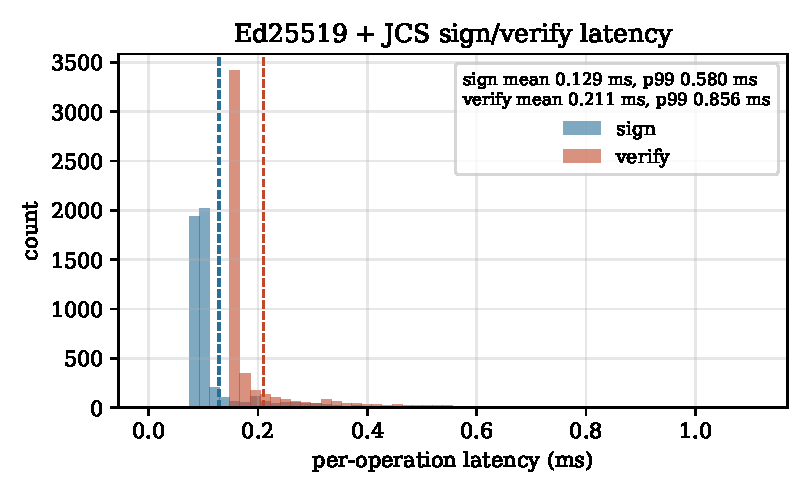
\includegraphics[width=0.72\textwidth]{figures/verify_latency.pdf}
\caption{Per-operation latency distribution for the sign and verify paths (JCS
canonicalization plus Ed25519), 5000 iterations each. Dashed lines mark the
means. Both paths are sub-millisecond in the body of the distribution, with a
short scheduler-induced tail.}
\label{fig:latency}
\end{figure}

\begin{figure}[h]
\centering
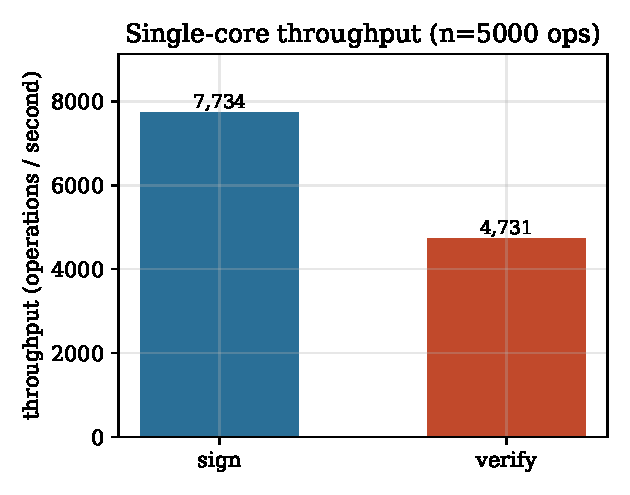
\includegraphics[width=0.52\textwidth]{figures/throughput.pdf}
\caption{Single-core throughput for the sign and verify paths. Verification is
the hot path for a relying party; at roughly $4{,}700$ verifies/s per core the
record cryptography is not the bottleneck relative to the external attestation
and transparency lookups a full appraisal also performs.}
\label{fig:throughput}
\end{figure}

\subsection{Record size}

Trust Records are compact. Table~\ref{tab:eval-size} gives the canonical
(signature pre-image) size of each shipped vector plus a synthetic, fully
populated Level~2 record. A minimal Level~0 record is under $0.9$~KB; a complete
Level~2 record with TEE measurement, SLSA provenance, tool-transcript binding,
and transparency receipt is under $1.4$~KB; the cMCP-profiled envelope, which
carries the full gateway call summary, is $1.6$~KB. The synthetic record was
measured with the v0.1 profile URI; the committed harness now emits the v0.2
URI, which is four bytes longer, and gives 1{,}389 bytes. Records this small travel with
the workload as a header or sidecar without meaningful overhead.

\begin{table}[h]
\centering
\small
\caption{Canonical (JCS, signature pre-image) size of the shipped conformance
vectors and a synthetic fully-populated Level~2 record, from
\texttt{experiments/results/record\_sizes.json}.}
\label{tab:eval-size}
\begin{tabular}{lr}
\toprule
Record & canonical size (bytes) \\
\midrule
\texttt{valid\_level0} (minimal L0)        & 878 \\
\texttt{valid\_level0\_with\_transcript}   & 1{,}109 \\
synthetic full L2 (all fields)             & 1{,}385 \\
\texttt{valid\_cmcp\_runtime} (cMCP profile) & 1{,}612 \\
\bottomrule
\end{tabular}
\end{table}

\subsection{Conformance suite behaviour}

Finally we ran the shipped \texttt{trace-tests} runner over every shipped vector
at Levels~0, 1, and 2, tallying \texttt{pass}/\texttt{fail}/\texttt{skip}/%
\texttt{unverified} findings (Table~\ref{tab:eval-conf}). The archival vectors
are unsigned test data with a 2025 \texttt{iat}, so the run disables the freshness
bound to isolate \emph{structural} conformance; TR-SIG correspondingly reports
\texttt{unverified} for the unsigned plain-trace vectors, which is the honest
expected outcome (an \texttt{unverified} record passes at Level~0 with an advisory
and fails at Level~1 and above, per Section~\ref{sec:conformance}). The two plain-trace positive vectors pass at Level~0 and fail at
Levels~1 and~2. The cMCP fixture fails at all three levels in this captured run.
The \texttt{invalid\_wrong\_profile} fixture fails at every level, while
\texttt{invalid\_missing\_runtime} passes at Level~0 and fails at Levels~1 and~2.
These are the outcomes in the committed result JSON; fixture names do not
establish the expected or observed verdict. In particular, the Level~0 pass
for the missing-runtime fixture is a limit of this historical check set,
not evidence of complete structural validation. The signed-record path is
exercised separately by the sign/verify benchmark. These results describe
the recorded package versions and do not certify the current implementation.

\begin{table}[h]
\centering
\small
\caption{Conformance findings from the shipped \texttt{trace-tests} runner
(\texttt{experiments/results/conformance.json}), reported as
pass\,/\,fail\,/\,skip\,/\,unverified. ``L0 pass'' is the suite's overall verdict
at Level~0. Freshness disabled to isolate structural conformance of the archival
vectors; unsigned plain-trace vectors report TR-SIG \texttt{unverified} by design.}
\label{tab:eval-conf}
\begin{tabular}{llccc}
\toprule
Vector & fmt & L0 (p/f/s/u) & L1 (p/f/s/u) & L2 (p/f/s/u) \\
\midrule
\texttt{valid\_level0}              & trace & 7/0/0/1 & 11/1/1/0 & 12/2/1/0 \\
\texttt{valid\_level0\_w/transcript} & trace & 7/0/0/1 & 11/1/1/0 & 14/1/1/0 \\
\texttt{valid\_cmcp\_runtime}       & cMCP  & 6/1/0/0 & 8/2/1/0  & 10/3/1/0 \\
\texttt{invalid\_missing\_runtime}  & trace & 7/0/0/1 & 9/2/0/0  & 10/3/0/0 \\
\texttt{invalid\_wrong\_profile}    & trace & 6/1/0/1 & 10/2/1/0 & 11/3/1/0 \\
\bottomrule
\end{tabular}
\end{table}

\section{Related Work}
\label{sec:related}

\paragraph{Attestation standards.}
TRACE composes rather than replaces. It instantiates RATS~\citep{rats2021} and
profiles EAT~\citep{eat2023} for the wire envelope; where platform SDKs (AMD
SEV-SNP~\citep{amdsevsnp2023}, Intel TDX~\citep{inteltdx2023}, and GPU/cloud
attestation services) each emit their own evidence shape, TRACE maps that evidence
into one envelope and adds the governance, identity, and audit claims an agent
runtime needs. Unlike a bare platform quote, a Trust Record answers \emph{what ran},
\emph{under what policy}, \emph{on what data}, and \emph{invoking which tools}, not
merely \emph{that the environment is genuine}.

\paragraph{Supply-chain and identity.}
TRACE references SLSA provenance for build-time integrity, SPIFFE~\citep{spiffe2018}
for workload identity bound to the TEE measurement, and AIBOM formats (SPDX/CycloneDX)
for component inventory, each by digest from the corresponding claim. The
companion Agent Manifest specification~\citep{manifest2026} extends identity to the
full set of agent-defining artifacts.

\paragraph{Tamper-evident logs.}
The audit commitment and the \texttt{transparency} receipt build on certificate
transparency~\citep{ct2013}, secure audit logging~\citep{seclog2000}, and the SCITT
append-only-log model. TRACE differs in scoping the per-session chain, binding its
tip into a hardware-attested record, and registering the record on a transparency
log, so a registered record cannot later be altered or replaced
unnoticed. Registration alone does not reveal omitted events; that requires an
independently expected event set or terminal boundary (Section~\ref{sec:conclusion}).

\paragraph{Agent governance.}
Output-filtering and guardrail frameworks constrain agent inputs and outputs but do
not attest \emph{that} enforcement occurred or under which policy. AGT~\citep{agt2026}
supplies the policy engine and identity layer; TRACE is the hardware-attested
evidence those controls produce, verifiable by a third party after the fact.

\section{Conclusion}
\label{sec:conclusion}

TRACE gives AI agent runtimes a portable, hardware-attestable evidence record, the
Trust Record, that a relying party can appraise offline, without trusting the
operator. By instantiating the RATS roles and profiling EAT, it reuses established
attestation machinery while adding the model, runtime, policy, data-class,
tool-transcript, provenance, appraisal, and transparency claims an agent deployment
must account for. A confirmation key identifies the signing key; verified attestation must bind
that key to a hardware root before silicon provenance can be claimed. The signed
body makes modification detectable. An inclusion proof establishes membership
in a particular tree, not completeness of execution or absence of omitted events.
Completeness requires an independently expected event set or terminal boundary.
The historical fixture outcomes in Section~\ref{sec:eval} also show limits of
the software conformance checks.

\paragraph{Limitations and future work.}
The base format is settled, but several pieces are deliberately staged. Silicon
cert-chain appraisal (AMD KDS, Intel DCAP) is an online step a fully offline verifier
reports as unverified rather than fatal. The external-execution-evidence receipt
format (Section~\ref{sec:model}) is specified but not yet exercised by the conformance
suite. Profile coverage is growing: cMCP is the reference profile at the MCP boundary,
with A2A and additional platform profiles planned. As more profiles and vendor
attestation surfaces are mapped in, the registry and conformance levels give the
ecosystem a shared, testable definition of what a trustworthy agent execution record
is.


\bibliographystyle{plainnat}
\bibliography{refs}

\end{document}
